\documentclass[pdf]{beamer}
\usetheme{Copenhagen}
\usepackage{multicol, latexsym, amsmath, amssymb}
\usepackage{smartdiagram}
\usepackage{subcaption}

\setbeamertemplate{navigation symbols}{}
\newcommand{\z}{\mathbf{z}}
\newcommand{\uout}{u_{out}}
\newcommand{\vout}{v_{out}}
\newcommand{\uoutdum}{u_{out}^{dum}}
\newcommand{\uinplus}{u_{in}^{+}}
\newcommand{\uinminus}{u_{in}^{-}}
\newcommand{\winl}{w_{in}^{l}}
\newcommand{\win}{w_{in}}
\newcommand{\uin}{w_{in}}
\newcommand{\vin}{v_{in}}

\DeclareMathOperator*{\plusrightarrow}{\ensuremath{\xrightarrow{+}}}
\DeclareMathOperator*{\minusrightarrow}{\ensuremath{\xrightarrow{-}}}
\DeclareMathOperator*{\plusleftarrow}{\ensuremath{\xleftarrow{+}}}
\DeclareMathOperator*{\minusleftarrow}{\ensuremath{\xleftarrow{-}}}

\title{Variational Bayesian Unlearning}
\subtitle[]{Quoc Phong Nguyen, Bryan Kian Hsiang Low, and Patrick Jaillet}

\author[Nguyen et al]{Presented by Ananth Mahadevan}
\date{\today}

\begin{document}
\begin{frame}
    \titlepage
\end{frame}

\begin{frame}
    \frametitle{Contents}
    \tableofcontents
\end{frame}

\begin{frame}
  \frametitle{Bayesian Basics}
  \textbf{Learning}
  \begin{itemize}
    \item Unknown model parameters $\bm{\theta}$ 
    \item Prior belief $p(\bm{\theta})$ 
    \item Set $\da$ of training data
    \item Learn approximate posterior belief $q(\bm{\theta}|\da) \approx p(\bm{\theta}|\da)$ 
  \end{itemize}
  \textbf{Unlearning}
  \begin{itemize}
    \item $\da$ partitioned into $\dr$ \emph{erased data} and $\dc$ of \emph{remaining data} 
    \item $\da = \dc\ \cup\ \dr$ and $\dc\ \cap\ \dr = \emptyset$. 
    \item Approximate $p(\bm{\theta}|\dc)$ 
  \end{itemize}
\end{frame}

\begin{frame}<1>[label=overview]
  \frametitle{Overview}
  \begin{figure}
    \centering
\tikzstyle{textblock} = [rectangle, text width=4em, text centered, line width=1pt]
\tikzstyle{block} = [rectangle, draw, fill=uablue25, 
    text width=4em, text centered, rounded corners, minimum height=2em, line width=1pt ]
\tikzstyle{line} = [line width=1pt, -triangle 45]
\tikzstyle{alert} = [text=uared100, fill=uared25, draw=uared100]
\tikzstyle{normal} = [text=uablue100, fill=uablue25, draw=uablue100]
\tikzstyle{dim} = [text=uablue25, fill=uablue5, draw=uablue25]
\tikzstyle{hide} = [draw=None]

\begin{tikzpicture}[node distance=1.5cm, auto]
    % Place nodes
    \node [textblock] (original) {Original Model};
    \node [textblock] (target) [right of=original, node distance=4cm] {Target Model};

    \node [textblock] (unlearn) [right of=target, node distance=4cm] {Unlearned Model};

    \node [block,onslide=<2->{dim},temporal=<2-3>{}{alert}{dim},temporal=<5-8>{}{alert}{dim},temporal=<9>{}{normal}{dim}] (posterior) [below of=original, node distance=2cm] {$\ex(\param|\data)$};

    \node [block,onslide=<2->{dim},temporal=<3-5>{}{alert}{dim},temporal=<9>{}{normal}{dim}] (retrain) [below of=target, node distance=2cm] {$\ex(\param|\remain)$};

    \node [block,onslide=<2->{dim},temporal=<4-5>{}{alert}{dim},temporal=<9>{}{normal}{dim}] (qu) [below of=unlearn, node distance=2cm] {$\un(\param|\remain)$};

    \node [block,onslide=<2->{dim},temporal=<2>{}{alert}{dim},temporal=<6-8>{}{alert}{dim},temporal=<9>{}{normal}{dim}] (posapp) [below of=posterior, node distance=2cm] {$\posapp(\param|\data)$};

    \onslide<-6>{
    \node [block,onslide=<2->{dim},temporal=<6>{}{alert}{dim}] (tarapp) [below of=retrain, node distance=2cm] {$\exapp(\param|\remain)$};

    \node [block,onslide=<2->{dim},temporal=<6>{}{alert}{dim}] (unapp) [below of=qu, node distance=2cm] {$\unapp(\param|\remain)$};
    }
    
    \onslide<7->{
        \node [block,onslide=<2->{dim},temporal=<7>{}{alert}{dim},temporal=<9>{}{normal}{dim}] (tarappadj) [below of=retrain, node distance=1cm] {$\exapp_{\text{adj}}(\param|\remain)$};

        \node [block,onslide=<2->{dim},temporal=<8>{}{alert}{dim},temporal=<9>{}{normal}{dim}] (tarapp2) [below of=retrain, node distance=3cm] {$\exapp(\param|\remain)$};

        \node [block,onslide=<2->{dim},temporal=<7>{}{alert}{dim},temporal=<9>{}{normal}{dim}] (unappadj) [below of=qu, node distance=1cm] {$\unapp(\param|\remain)$};
    
        \node [block,onslide=<2->{dim},temporal=<8>{}{alert}{dim},temporal=<9>{}{normal}{dim}] (rkl) [below of=unappadj, node distance=2cm] {$\rklapp(\param|\remain)$};
    }
    
    % % Draw edges
    \draw [line,onslide=<2->{dim},temporal=<2>{}{alert}{dim},temporal=<6-8>{}{alert}{dim},temporal=<9>{}{normal}{dim}] (posapp.north) -> (posterior.south) node [midway, left] (TextNode) {$\mathcal{L}$};
    \draw [line,onslide=<2->{dim},temporal=<4>{}{alert}{dim},temporal=<9>{}{normal}{dim}] (qu.west) -> (retrain.east) node [midway,above] (eubo) {$\mathcal{U}$};

    \onslide<-6>{
    \draw [line,onslide=<2->{dim},temporal=<6>{}{alert}{dim},temporal=<9>{}{normal}{dim}] (unapp.west) -> (tarapp.east) node [midway,above] (euboapp) {$\tilde{\mathcal{U}}$}; 
    \draw [line,onslide=<2->{dim},temporal=<6>{}{alert}{dim},temporal=<9>{}{normal}{dim}] (tarapp.west) -> (posapp.east) node [midway, above] {Bayes' Rule};
    }
    \onslide<7->{
        \draw [line,onslide=<2->{dim},temporal=<7>{}{alert}{dim},temporal=<9>{}{normal}{dim}] (unappadj.west) -> (tarappadj.east) node [midway,below] (euboapp) {$\tilde{\mathcal{U}_{\text{adj}}}$};     
    
        \draw [line,onslide=<2->{dim},temporal=<8>{}{alert}{dim},temporal=<9>{}{normal}{dim}] (rkl.west) -> (tarapp2.east) node [midway,below] (rKL) {rKL};

        \draw [line,onslide=<2->{dim},temporal=<7>{}{alert}{dim},temporal=<9>{}{normal}{dim}] (tarappadj.west) -> (posapp.east);

        \draw [line,onslide=<2->{dim},temporal=<8>{}{alert}{dim},temporal=<9>{}{normal}{dim}] (tarapp2.west) -> (posapp.east) node [midway, above right=0.cm,temporal=<7>{}{color=uared100}] {Bayes' Rule};
    }
    \draw [line,onslide=<2->{dim},temporal=<3>{}{alert}{dim},temporal=<9>{}{normal}{dim}] (retrain.west) -> (posterior.east) node [midway, above] {Bayes' Rule};

\end{tikzpicture}
\end{figure}
\end{frame}

\section{Learning}

\subsection{VI and ELBO}
\againframe<2>{overview}

\begin{frame}
  \frametitle{Evidence Lower Bound (ELBO)}
  \begin{itemize}
    \item Need to \textbf{minimize} the KL divergence $\text{KL}[q(\bm{\theta}|\da)\ \Vert\  p(\bm{\theta}|\da)] \triangleq \int q(\bm{\theta}|\da)\ \log (q(\bm{\theta}|\da) / p(\bm{\theta}|\da))\ \text{d}\bm{\theta}$
    \item Or, \textbf{maximize} the \emph{evidence lower bound} (ELBO) 
    \[
      \mcl{L} \triangleq \int \underbrace{q(\bm{\theta}|\da)\ \log p(\da | \bm{\theta})\ \text{d}\bm{\theta}}_{\text{increase likelihood}} - \underbrace{\text{KL}[q(\bm{\theta}|\da)\ \Vert\ p(\bm{\theta})]}_{\text{remember prior}}
    \]
    \item Use \textbf{Black Box Variational Inference} (BBVI) if  $\mcl{L}$ cannot be evaluated in closed form
    \begin{itemize}
      \item Stochastic gradient estimates for Gradient Ascent
    \end{itemize}
  \end{itemize}
\end{frame}

\section{Unlearning}
\subsection{Exact}
\againframe<3>{overview}
\begin{frame}
  \frametitle{Exact Bayesian Unlearning}
  \begin{itemize}
    \item Retraining on $\dc$ we can get $p(\bm{\theta}|\dc)$, but computationally costly,
    \item Alternatively, using Bayes' rule 
    \[
      p(\bm{\theta}|\dc)\ \ =\ \  {p(\bm{\theta}|\da) \ p(\dr|\dc)}/{p(\dr| \bm{\theta})}
%, \dc
	\ \ \propto\ \  {p(\bm{\theta}|\da)}/{p(\dr| \bm{\theta})} 
    \]
    \item For discrete $\param$ and conjugate priors can be obtained directly
    \item Paper focuses on \textbf{non-conjugate priors}
  \end{itemize}
  

\end{frame}
\subsection{EUBO}
\againframe<4>{overview}
\begin{frame}
  \frametitle{Approximate Bayesian Unlearning}
  \begin{itemize}
    \item Find $q_u(\bm{\theta}|\dc) \approx p(\bm{\theta}|\dc)$ by unlearning from erased data $\dr$
    \item Predictive distributions
    \begin{itemize}
      \item $q_u(y|\dc) \triangleq %\mbb{E}_{q_u(\bm{\theta}|\dc)}[p(\mbf{y}|\bm{\theta})] = 
      \int p(y|\bm{\theta})\ q_u(\bm{\theta}|\dc)\  \text{d}\bm{\theta}$
      \item $p(y|\dc) = %\mbb{E}_{p(\bm{\theta}|\dc)}[p(\mbf{y}|\bm{\theta})] = 
      \int p(y|\bm{\theta})\ p(\bm{\theta}|\dc)\  \text{d}\bm{\theta}$
    \end{itemize}
    \item Loss to minimize: $\text{KL}[q_u(y|\dc)\ \Vert\ p(y|\dc)]$
    \begin{itemize}
      \item Closed form may not exist
      \item Hard to estimate and optimize
    \end{itemize}
  \end{itemize}
  \begin{block}<2->{Propostion 1 Bound}
    $$\text{KL}[q_u(y|\dc)\ \Vert\ p(y|\dc)] \le \text{KL}[q_u(\bm{\theta}|\dc)\ \Vert\ p(\bm{\theta}|\dc)]$$
  \end{block}
  \begin{itemize}
    \item<2-> How to \textbf{minimize} $\text{KL}[q_u(\bm{\theta}|\dc)\ \Vert\ p(\bm{\theta}|\dc)]$ ?
  \end{itemize}
\end{frame}

\begin{frame}
  \frametitle{Evidence Upper Bound (EUBO)}
  \begin{itemize}
    \item Similar to ELBO define an \emph{evidence upper bound}
    \[
      \mcl{U} \triangleq \int \underbrace{q_u(\bm{\theta}|\dc)\ \log p(\dr|\bm{\theta})\ \text{d}\bm{\theta}}_{\text{Forget }\dr} + \underbrace{\text{KL}[q_u(\bm{\theta}|\dc)\ \Vert\ p(\bm{\theta}|\da)]}_{\text{Remember } \da (\text{incudes }\dc)} 
    \]
    \item We can minimize $\text{KL}[q_u(\bm{\theta}|\dc)\ \Vert\ p(\bm{\theta}|\dc)]$ in two ways
    \begin{enumerate}
      \item \textbf{Maximize} ELBO while retraining using $\dc$ 
      \item \textbf{Minimize} EUBO when unlearning with $\dr$
    \end{enumerate}
    \item EUBO naturally has regularizing term to avoid \emph{catastrophic forgetting}
  \end{itemize}
  

\end{frame}

\begin{frame}
  \frametitle{EUBO and ELBO}
  \begin{figure}
    %\centering
    \begin{tabular}{c}
         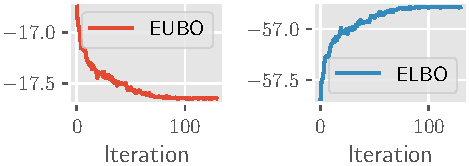
\includegraphics[height=0.17\textwidth]{paper/img/train_eubo.pdf}\\
         (a) Unlearning from $\dr$ by minimizing EUBO\\
         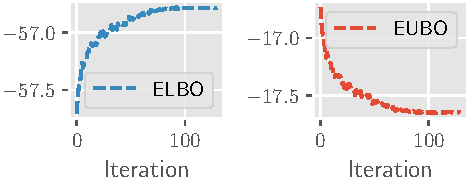
\includegraphics[height=0.17\textwidth]{paper/img/train_elbo.pdf}\\
         (b) Retraining with $\dc$ by maximizing ELBO
    \end{tabular}
    \caption{Plots of EUBO and ELBO when (a) unlearning from $\dr$ and (b) retraining with $\dc$.}
    \label{fig:eubovselbo}
    \end{figure}
\end{frame}

\againframe<5>{overview}

\subsection{Adjusted EUBO}
\begin{frame}
  \frametitle{Reality Check}
  \begin{itemize}
    \item In reality we only obtain approximations
    \item VI training gives approximate posterior $q(\bm{\theta}|\da)$ 
    \item We can estimate unknown $p(\bm{\theta}|\dc)$ using 
    \[
      \tilde{p}(\bm{\theta}|\dc)\ \  \propto\ \ {q(\bm{\theta}|\da)}/{p(\dr| \bm{\theta})}
    \]
    \item $\eubo(\bm{\theta}|\dc)$ from minimizing loss $\text{KL}[\eubo(\bm{\theta}|\dc)\ \Vert\ \tilde{p}(\bm{\theta}|\dc)]$
    \item Define following EUBO
    \[
      \widetilde{\mcl{U}} \triangleq \int \eubo(\bm{\theta}|\dc)\ \log p(\dr|\bm{\theta})\ \text{d}\bm{\theta} + \text{KL}[\eubo(\bm{\theta}|\dc)\ \Vert\ q(\bm{\theta}|\da)]  
    \]
    \end{itemize}
\end{frame}

\againframe<6>{overview}

\begin{frame}
  \frametitle{Issues}
  Two possible sources of inaccuracy in $q(\bm{\theta}|\da)$
  \begin{enumerate}
    \item $q(\bm{\theta}|\da)$ often underestimates the variance of $p(\bm{\theta}|\da)$
    \item Unlikely that the ELBO is maximized using samples of $\bm{\theta}$ with small $q(\bm{\theta}|\da)$
  \end{enumerate}
  Hence, curb unlearning at values of $\bm{\theta}$ with small $q(\bm{\theta}|\da)$
  \begin{figure}
    \centering
    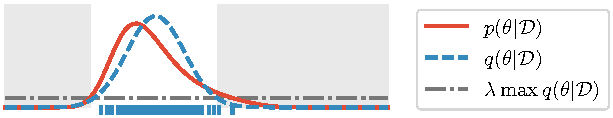
\includegraphics[width=0.63\textwidth]{paper/img/vi_ep.pdf}
    \caption{Plot of  $q(\bm{\theta}|\da)$ learned using VI. Gray shaded region corresponds to values of $\bm{\theta}$ where $q(\bm{\theta}|\da) \le \lambda \max_{\bm{\theta}'} q(\bm{\theta}'|\da)$. Vertical blue strips on  horizontal axis show $100$ samples of $\bm{\theta} \sim q(\bm{\theta}|\da)$.}
    \label{fig:adjustedvi}
    \end{figure}
\end{frame}

\againframe<7>{overview}

\begin{frame}
  \frametitle{Adjusted EUBO}
    Introduce $\lambda \in [0,1]$ to control focus of unlearning
    \[
      p_{\text{adj}}(\dr|\bm{\theta}; \lambda) \triangleq 
	\begin{cases}
		p(\dr|\bm{\theta}) &\text{ if } q(\bm{\theta}|\da) > \lambda \max_{\bm{\theta}'} q(\bm{\theta}'|\da)\ ,\\
		1 &\text{ otherwise (i.e., shaded area )}\ ;
		%&\text{ if } q(\bm{\theta}|\da) \le \lambda \max_{\bm{\theta}'} q(\bm{\theta}'|\da)
	\end{cases}
    \]
    \[
      \tilde{p}_{\text{adj}}(\bm{\theta}|\dc; \lambda) \propto 
	\begin{cases}
		q(\bm{\theta}|\da) / p(\dr| \bm{\theta}) &\text{ if } q(\bm{\theta}|\da) > \lambda \max_{\bm{\theta}'} q(\bm{\theta}'|\da)\ ,\\
		q(\bm{\theta}|\da) &\text{ otherwise (i.e., shaded area )\ }
		%&\text{ if } q(\bm{\theta}|\da) \le \lambda \max_{\bm{\theta}'} q(\bm{\theta}'|\da)
	\end{cases}
    \]
    \[
      \widetilde{\mcl{U}}_{\text{adj}}(\lambda) \triangleq \int \eubo(\bm{\theta}|\dc; \lambda)\ \log p_{\text{adj}}(\dr|\bm{\theta}; \lambda)\ \text{d}\bm{\theta} + \text{KL}[\eubo(\bm{\theta}|\dc; \lambda)\ \Vert\ q(\bm{\theta}|\da)]
    \]
  
\end{frame}

\subsection{Reverse KL}
\againframe<8>{overview}
\begin{frame}
  \frametitle{Reverse KL}
  \begin{itemize}
    \item Minimize $\text{KL}[\tilde{p}(\bm{\theta}|\dc)\ \Vert\ \elbo(\bm{\theta}|\dc)]$ instead
    \item Now, $\elbo(\bm{\theta}|\dc)$ \textbf{overestimates} the variance of $\tilde{p}(\bm{\theta}|\dc)$
    \item Initialize $\elbo(\bm{\theta}|\dc)$ at $q(\bm{\theta}|\da)$ for faster convergence
    \item Now, SGA naturally curbs unlearning at values of $\bm{\theta}$ with small $q(\bm{\theta}|\da)$
  \end{itemize}

\end{frame}

\begin{frame}
  \frametitle{Adjusted EUBO and rKL}
  \begin{figure}
    \centering
    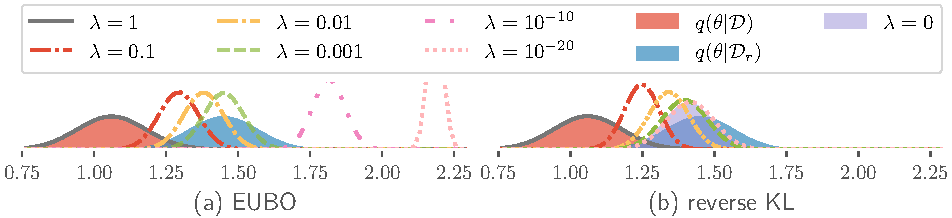
\includegraphics[width=\textwidth]{paper/img/gamma_unknown_mean/gamma_unlearn.pdf}
    \caption{Plot of approximate posterior beliefs with varying $\lambda$ obtained by minimizing (a) EUBO (i.e., $\eubo(\bm{\theta}|\dc;\lambda)$) and (b) reverse KL (i.e., $\elbo(\bm{\theta}|\dc;\lambda)$); horizontal axis denotes $\theta = \alpha$.
    In (a), a huge probability
    %the majority of the
    mass of $\eubo(\bm{\theta}|\dc, \lambda=0)$ is at large values of $\alpha$ beyond the plotting area and the top of the plot of $\eubo(\bm{\theta}|\dc, \lambda=10^{-20})$ is cut off due to lack of space.
    }
    \label{fig:expunlearn}
    \end{figure}
\end{frame}

\againframe<9>{overview}
\section{Results}
\begin{frame}
  \frametitle{Reults}

  
\end{frame}




\end{document}  

% \begin{frame}{Introductory stuff}
% \begin{itemize}[<+->]
% \item Stuff
% \item Stuff
% \item Stuff
% \item Stuff
% \end{itemize}
% \end{frame}

% \againframe<2>{overview}

% \begin{frame}{Stuff about VFH}
% \begin{itemize}[<+->]
% \item Stuff
% \item Stuff
% \item Stuff
% \item Stuff
% \item Stuff
% \end{itemize}
% \end{frame}

% \againframe<3>{overview}

% \begin{frame}{Stuff about Robot}
% \begin{itemize}[<+->]
% \item Stuff
% \item Stuff
% \item Stuff
% \end{itemize}
% \end{frame}

% \end{document}